\label{sec:power-bpo-algorithm}

本节在第~\ref{sec:power-setup}~节定义的单教师、单 rollout 和冻结前缀测度上拟合 target。外层锚点 $q_n$ 与教师信号冻结，内层学生 $p_{n,j}$ 及其条件中心随参数更新。所有微分均不穿过 rollout、前缀权重、锚点与教师。

\subsection{形状参数只进入冻结监督信号}

使用式~\eqref{eq:proximal-power-signal} 与式~\eqref{eq:center-explicit-definition} 的冻结 $f,A$。目标构造已经由前两节证明，下面将它接到 BPO 的条件回归目标。

从下面的 KL mirror 子问题开始：
\begin{equation}
 m=\argmax_{p\in\Delta}
 \left\{\sum_a p_a A_{\kappa,\eta}(a)
       -\frac1\eta\KL(p\Vert q)\right\}.
 \label{eq:power-bpo-mirror-subproblem}
\end{equation}
根据第~\ref{thm:power-md-integrable-objective}~定理，其唯一解为
\begin{equation}
 m_a=q_ae^{f_a}/Z,\qquad Z=\sum_bq_be^{f_b}.
 \label{eq:power-bpo-explicit-target}
\end{equation}
改变 $\kappa$ 改变冻结监督和 target；KL 正则仍为 $\KL(p\Vert q)$。BPO 内层拟合这个 target，通常不直接最小化重心目标 $F$ 或教师目标 $\mathcal J$。

\subsection{BPO 损失、中心和精确梯度}

令 $C_qh=h-\E_qh$，定义
\begin{align}
 b_\theta&=\E_q[U_\theta-f],\\
 R_\theta(a)&=U_\theta(a)-f_a-b_\theta
            =C_q\log(p_\theta/m)_a,\\
 \mathcal L_n(\theta)
 &=\E_{s\sim\widehat d_n}\frac1{2\eta}
     \E_{a\sim q_n(\cdot\mid s)}R_\theta(s,a)^2.
 \label{eq:power-bpo-population-loss}
\end{align}
等价地，令 $\delta=C_q[U_\theta/\eta-A]$，则 $\mathcal L_n=(\eta/2)\E_{\widehat d_n,q}\delta^2$。$\kappa=0$ 时正好恢复原 BPO 的归一化损失。$\log Z$ 被 $C_q$ 消掉，因此无需显式计算 target 的归一化常数。teacher 监督只需本轮缓存 $f$ 及 $\E_qf$；学生项 $\E_qU_\theta$ 必须随 inner 参数更新，不能连同 teacher 中心一起冻结。

对固定 prefix，$\psi_\theta(a)=\nabla_\theta\log p_\theta(a)$。由于 $\nabla b_\theta=\E_q\psi_\theta$ 与 $\E_qR_\theta=0$，直接微分得到
\begin{align}
 \nabla_\theta\mathcal L_s
 &=\frac1\eta\E_q[R_\theta(\psi_\theta-\E_q\psi_\theta)]\\
 &=\frac1\eta\E_q[R_\theta\psi_\theta].
 \label{eq:power-bpo-gradient}
\end{align}
所以精确 BPO 不带 $p/q$ 重要性比率；测度就是冻结 $q$。若使用随机 action 估计最后一个期望，系数 $\sg(R_\theta/\eta)$ 乘以 $\log p_\theta(a)$ 给出所需 score 梯度。若直接微分完整平方损失，中心可以正常参与自动微分，其导数因精确零均值而抵消；两种停止梯度语义不能混为一谈。

用已定义的冻结中心 $K$ 展开 BPO 系数，得到
\begin{equation}
 \frac{R(a)}\eta
 =\frac{U(a)+\KL(q\Vert p)}\eta-A_{\kappa,\eta}(a)-K_{\kappa,\eta}.
\end{equation}
因此需要同时替换 action 监督 $r\mapsto A$ 和冻结教师中心 $\KL(q\Vert T)\mapsto K_{\kappa,\eta}$；只改变 action 监督却沿用原教师中心会产生偏差。$\kappa=0$ 时 $K_{0,\eta}=\KL(q\Vert T)$，恢复原接口。一般 $\kappa$ 下，由 $\E_qf=-\KL(q\Vert m)+\log Z$，有 $K_{\kappa,\eta}=[\KL(q\Vert m)-\log Z]/\eta$，它不是原 teacher KL。学生中心仍是当轮不断重算的 $\KL(q\Vert p)$。

完整支持下 $\mathcal L_s=0$ 当且仅当 $\log(p_a/m_a)$ 对全部 action 是常数。归一化强制该常数为零，因此 $p=m$。多 prefix、共享参数时，零损失还要求网络能同时表示全部条件 target；不可实现时只是 BPO 投影，不能宣称等于理想 mirror 更新。
\subsection{完整词表求和与一条轨迹的 action 估计}

一条 rollout 足以给出训练前缀，并不要求损失只使用每个前缀实际生成的一个 token。若能访问该前缀完整 $q,T,p$ 概率，可以直接求式~\eqref{eq:power-bpo-population-loss} 的 action 期望，仍然只有一次 response 生成，没有辅助 rollout 或候选组。这是本节的精确参考算法。

若只使用 rollout 中的 action，估计量为 $g(a)=R_\theta(a)\psi_\theta(a)/\eta$。对固定的 $s,\theta$ 和独立 $a\sim q(\cdot\mid s)$，它无偏。只用这一 action 同时估计本前缀的中心会令 $R=0$，使算法退化；把一条 response 的不同前缀 token 当作同一条件分布的组均值，也不能得到 $\E_{q(\cdot\mid s)}$。

复用整条已采样轨迹做 $I>1$ 个 inner 更新时，当前 $\theta$ 依赖已见 action，因而不再自动具有上述条件无偏性。给定固定样本 $a$，其平方残差损失的真正梯度是
\begin{equation}
 \nabla_\theta\frac{R_\theta(a)^2}{2\eta}
 =\frac{R_\theta(a)}\eta(\psi_\theta(a)-\E_q\psi_\theta),
\end{equation}
一般不等于停止系数的 $R_\theta(a)\psi_\theta(a)/\eta$。后者仍可作为 BPO population-gradient 的采样近似，但必须记录样本复用误差。对完整 rollout 的无偏性论证，还需 action 权重在抽取该 action 之前可确定；使用随机最终长度作分母是比率估计，不能直接套用逐条件无偏公式。完整词表求和对已冻结的经验前缀测度给出精确梯度，不受这些 action 估计问题影响。
\subsection{BPO 是带冻结测度的拟合损失}

对冻结 $q,m$，BPO population 损失是
\begin{equation}
 \mathcal L_{\mathrm{BPO}}(p;m,q)
 =\frac1{2\eta}\Var_q\!\left[\log\frac p m\right].
 \label{eq:divergence-map-bpo-loss}
\end{equation}
它一般不能写成仅以 $(p,m)$ 为自变量的 $D_g(p\Vert m)$。取二元词表，固定 $p,m$ 且 $\ell_1=\log(p_1/m_1)\ne\ell_2=\log(p_2/m_2)$，则
\begin{equation}
 \mathcal L_{\mathrm{BPO}}=\frac{q_1(1-q_1)}{2\eta}(\ell_1-\ell_2)^2.
\end{equation}
改变第三个分布 $q$ 会改变损失，任何固定生成函数的 $D_g(p\Vert m)$ 都不随 $q$ 改变。完整支持下，BPO 与 target 散度共享唯一零点 $p=m$，这一事实不意味着损失、曲率或有限步轨迹相同。

取切向扰动 $p=m+v$、$\sum_av_a=0$，并令全部 $v_a/m_a$ 一致趋零。展开 $\log(1+v_a/m_a)$ 得到
\begin{equation}
 \mathcal L_{\mathrm{BPO}}(m+v;m,q)
 =\frac1{2\eta}\left\{\sum_aq_a\frac{v_a^2}{m_a^2}
 -\left(\sum_aq_a\frac{v_a}{m_a}\right)^2\right\}
 +O\!\left(\max_a|v_a/m_a|^3\right).
\end{equation}
若 $q=m$，一次均值为 $\sum v=0$，二阶项恢复 $\sum v_a^2/m_a$ 的 Fisher 度量，另带 $1/\eta$。一般冻结 $q\ne m$ 时，BPO 的局部度量与 target 上的 Fisher 度量不同。若使用独立 logits $z$，则 $C_q\log(p/m)=C_q(z-\log m)$，全局 Hessian 为 $[\operatorname{diag}(q)-qq^\top]/\eta$，与 $\kappa$ 无关。

\subsection{BPO 的固定几何与有限 inner 性质}

令独立 logits 为 $z$，$p=\operatorname{softmax}(z)$。由于 $C_q$ 消掉 softmax 的归一化常数，单 prefix 损失成为
\begin{align}
 \mathcal L_s(z)&=\frac1{2\eta}
    (z-\log m)^\top Q_q(z-\log m),\\
 Q_q&=\operatorname{diag}(q)-qq^\top,\qquad
 \nabla_z\mathcal L_s=Q_q(z-\log m)/\eta,\\
 \nabla_z^2\mathcal L_s&=Q_q/\eta.
\end{align}
$Q_q$ 在常数方向为零，在 $\boldsymbol1^\perp$ 上正定。对 $v\perp\boldsymbol1$，
\begin{equation}
 v^\top Q_qv=\sum_aq_a(v_a-\E_qv)^2
 \ge q_{\min}\sum_a(v_a-\E_qv)^2
 \ge q_{\min}\|v\|^2.
\end{equation}
Gershgorin 界给出 $\lambda_{\max}(Q_q)\le\max_a2q_a(1-q_a)\le1/2$。独立 logits 的普通梯度下降因此在 $0<\alpha_{\mathrm{opt}}<2\eta/\lambda_{\max}(Q_q)$ 下收敛；$\alpha_{\mathrm{opt}}<4\eta$ 是充分条件。若 $h=z-\log m$ 的第 $i$ 个非零特征方向系数为 $c_i$，则
\begin{equation}
 \mathcal L_s(z_j)=\frac1{2\eta}\sum_i\lambda_i c_i^2
    (1-\alpha_{\mathrm{opt}}\lambda_i/\eta)^{2j}.
\end{equation}
这些是独立 logits 的精确结论，不是 AdamW 或共享神经网络的无条件收敛定理。固定 $q,\eta$ 时 $\kappa$ 完全不出现在 Hessian 中：它改变回归目标与起始残差，不改善这个二次问题的条件数。小 $\eta$ 会增大曲率，并不自动降低归一化后的起始梯度。

若 $\|\psi_\theta(a)\|\le S$，随机 action 梯度有
\begin{equation}
 \E_q\|g\|^2\le\frac{2S^2}{\eta}\mathcal L_s.
\end{equation}
在 $p=q$ 时 $R=-C_qf$，故 $\mathcal L_s(q)=\Var_q(f)/(2\eta)$。在可实现的 $p=m$ 处，每个 action 的残差和随机梯度都为零。因而 target 形状影响初始监督尾部，而 BPO 拟合本身提供残差下降时的噪声控制；两者承担不同作用。

BPO 损失下降并不自动意味着 teacher KL 或 $D_\kappa$ 下降。一个三元反例取 $q=(0.4999995,0.4999995,10^{-6})$、$T=(0.8,0.199999,10^{-6})$、$\eta=0.3$、$\kappa=0.5$。令 $p\propto m\exp(0,0,12)$。稀有 action 的 logit 误差由很小的 $q$ 权重计价，BPO 损失低于起点，却会显著提高 $\KL(p\Vert T)$。本节核验程序给出 $\mathcal L_s(q)=0.06227708$、$\mathcal L_s(p)=0.00024000$，而 $\KL(q\Vert T)=0.22314483$、$\KL(p\Vert T)=1.65421904$。因此有限 inner 仍需真 teacher 散度和拟合误差证书。

若在该 prefix 上控制 $\|R\|_\infty\le\epsilon$，记 $\ell=\log(p/m)=R+c$。由概率归一化 $c=-\log\E_me^R\in[-\epsilon,\epsilon]$，得到 $\|\ell\|_\infty\le2\epsilon$ 和 $\KL(p\Vert m)\le2\epsilon$。仅从 BPO 损失可保证 $\|R\|_\infty\le\sqrt{2\eta\mathcal L_s/q_{\min}}$，可以取这个上界为 $\epsilon$；大词表极小的 $q_{\min}$ 会使该保证很弱。这解释了精确最优点一致与有限拟合质量之间的差距。
\subsection{锚点 Fisher 预条件的 BPO 保留有限步镜像性质}

前面的反例允许任意候选 $p$。如果约束 inner 的实际路径，可以得到比零误差最优点更强的保证。仍使用独立 logits，令 $Q_q^+$ 为 $Q_q$ 的 Moore--Penrose 逆，采用冻结锚点 Fisher 预条件更新
\begin{align}
 z^+&=z-\gamma\eta Q_q^+\nabla_z\mathcal L_s
     =z-\gamma Q_q^+Q_q(z-\log m),\\
 p^+_a&\propto p_a^{1-\gamma}m_a^\gamma,\qquad 0<\gamma\le1.
 \label{eq:power-bpo-anchor-fisher-step}
\end{align}
由于 $Q_q^+Q_q$ 是 $\boldsymbol1^\perp$ 上的正交投影，它与恒等映射只差常数 logit；softmax 消掉该常数。因此上式是精确的分布恒等式。$Q_q$ 是锚点 $q$ 的 Fisher，不能改称当前 $p$ 的 Fisher。该更新也恰好等于以当前 $p$ 为 KL 正则参照、步幅 $\gamma$ 对固定拟合目标 $\KL(p\Vert m)$ 执行 entropy MD。这里的 KL 目标是本轮 $m$，不等于原教师目标 $T$。

从 $p_0=q$ 出发，允许每次 $0<\gamma_j\le1$，归纳得到
\begin{align}
 p_j&=p_{\xi_j},\qquad
 p_{\xi,a}=q_ae^{\xi f_a}/Z_\xi,\\
 \xi_j&=1-\prod_{h<j}(1-\gamma_h),\qquad
 \mathcal L_s(p_j)=(1-\xi_j)^2\mathcal L_s(q).
 \label{eq:power-bpo-finite-inner-path}
\end{align}
证明只需代入 $\log(p_\xi/q)=\xi f-\log Z_\xi$，于是 $R_\xi=-(1-\xi)C_qf$；再对几何插值的 log 密度求线性组合，得到 $\xi^+=\xi+\gamma(1-\xi)$。这个理想 inner 的损失收缩因子不依赖 $q_{\min}$ 或词表大小，因为预条件器消掉了 $Q_q$ 的非零谱；实际计算与神经网络可实现性另有成本。

\begin{theorem}[幂均值 BPO 镜像拟合路径的有限步 teacher 进展]
\label{thm:power-bpo-inner-all-f}
在完整正支持、$\kappa\in[0,1]$、$0<\eta\le1$ 下，对任意凸函数 $\Phi$、$\Phi(1)=0$，令
\begin{equation}
 D_\Phi(p\Vert T)=\sum_aT_a\Phi(p_a/T_a).
\end{equation}
沿 $p_\xi\propto qe^{\xi f}$、$0\le\xi\le1$，$D_\Phi(p_\xi\Vert T)$ 不增加。因而式~\eqref{eq:power-bpo-anchor-fisher-step} 从 $q$ 出发时，每个有限 inner 都不增加 teacher 双向 KL、总变差或平方 Hellinger 距离。
\end{theorem}

\begin{proof}
记 $r_a=\log(T_a/q_a)$。$f(r)$ 单调递增；当 $\kappa>0$ 时 $f'(r)=\eta e^{\kappa r}/(1-\eta+\eta e^{\kappa r})\le1$，$\kappa=0$ 时 $f'=\eta\le1$。于是
\begin{equation}
 u_{\xi,a}=\frac{p_{\xi,a}}{T_a}
 =\frac{\exp[-r_a+\xi f(r_a)]}{Z_\xi}
\end{equation}
作为 $r_a$ 的函数单调不增，因为 $-1+\xi f'(r)\le0$。对于可微凸 $\Phi$，$\Phi'(u)$ 随 $u$ 单调不减，所以 $\Phi'(u_\xi(r))$ 随 $r$ 单调不增。微分归一化密度给出 $\partial_\xi p_\xi=p_\xi(f-\E_{p_\xi}f)$，因此
\begin{align}
 \frac{d}{d\xi}D_\Phi(p_\xi\Vert T)
 &=\operatorname{Cov}_{p_\xi}(\Phi'(u_\xi),f)\\
 &=\frac12\sum_{a,b}p_{\xi,a}p_{\xi,b}
   [\Phi'(u_{\xi,a})-\Phi'(u_{\xi,b})](f_a-f_b)
 \le0.
\end{align}
每个乘积非正，因为两因子对 $r$ 的单调性相反。有限词表和完整正支持下，$\{u_{\xi,a}:\xi\in[0,1],a\in\mathcal V\}$ 位于一个紧的正区间。任意有限凸函数都可在该区间由光滑凸函数一致逼近，逐点极限保留上述非增加关系，得到不可微情形。取 $\Phi(u)=u\log u$、$-\log u$、$|u-1|/2$ 与 $(\sqrt u-1)^2$，分别给出双向 KL、总变差与平方 Hellinger。\hfill$\square$
\end{proof}

对固定前缀测度逐条件求加权和保留该保证。任意降低 BPO 损失的候选则没有这项性质。共享神经网络、随机梯度、Fisher 近似和前缀测度刷新都可能离开指定路径，需要分别控制误差。

\begin{corollary}[通用单调信号 MD 的共同教师散度进展]
\label{cor:power-general-signal-all-f}
采用第~\ref{prop:power-general-signal-framework}~命题的 $S$，设 $L_S<\infty$、$0<\tau\le1/L_S$。则沿
\begin{equation}
 p_\xi\propto q\exp[\xi\tau S(T/q)],\qquad0\le\xi\le1,
\end{equation}
任意凸 $f$ 散度 $D_\Phi(p_\xi\Vert T)$ 都非增加。因此该步幅条件既保证对应教师目标 $\mathcal J_S$ 的 MD 下降，也保证其他凸生成教师散度不增加。
\end{corollary}

\begin{proof}
记 $r=\log(T/q)$、$f(r)=\tau S(e^r)$。则 $f'(r)=\tau e^rS'(e^r)\in(0,1]$。前一定理的证明仅使用 $f$ 单调递增和 $f'\le1$，未在协方差非正的论证中使用幂均值的其他性质，故逐步适用于此处的 $f$。
\end{proof}

\begin{figure}[htbp]
 \centering
 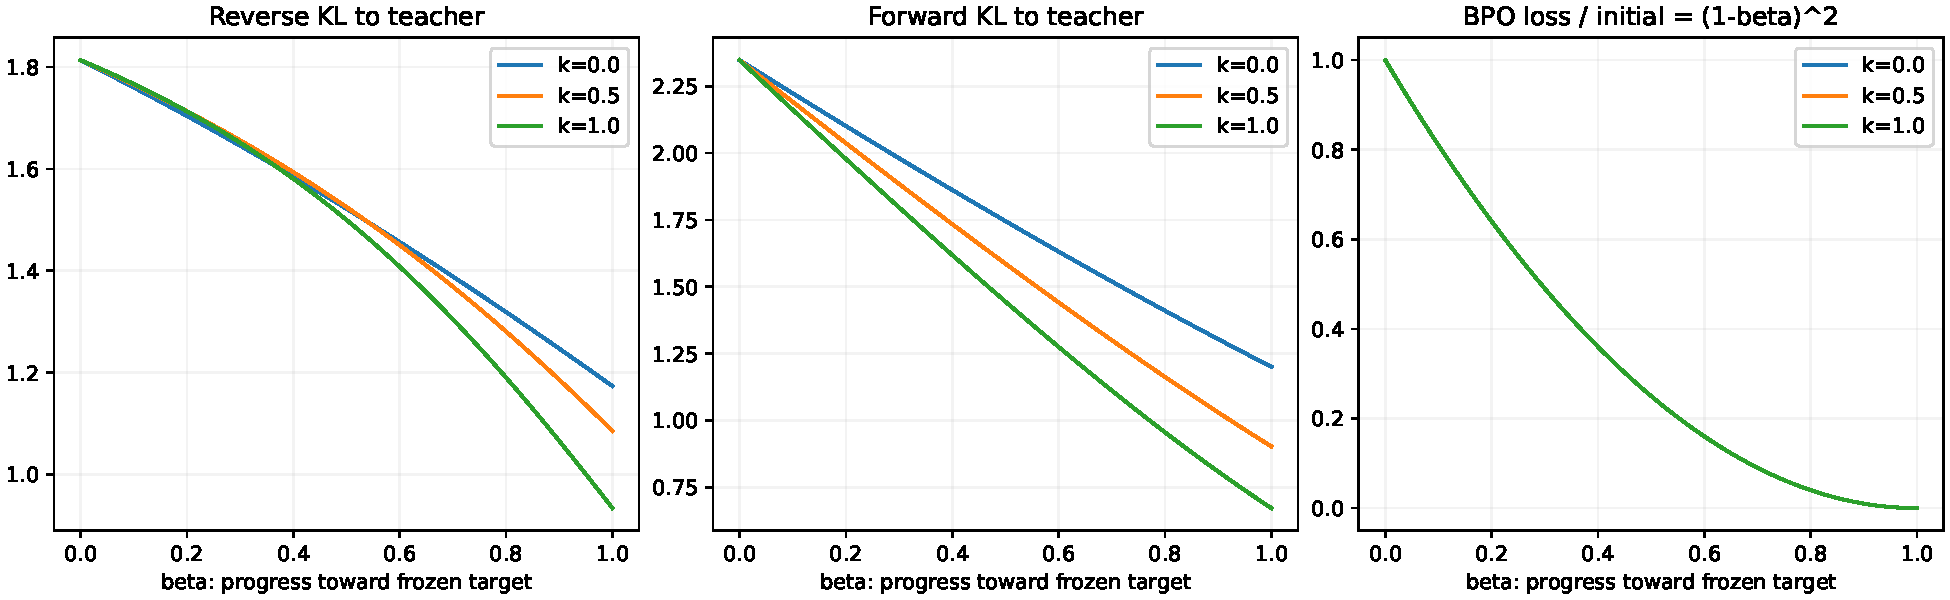
\includegraphics[width=\textwidth]{../../results/power-bpo-algorithm/finite-inner-progress.pdf}
 \caption{理想锚点 Fisher 预条件 BPO 的有限 inner：双向 teacher KL 沿 $\xi$ 下降，BPO 损失按 $(1-\xi)^2$ 精确收缩。图中旧记号 $\beta$ 对应本章 $\xi$；曲线为三元完整支持分布的解析求和。}
\end{figure}
\subsection{精确参考算法与实际 outer 更新}

\begin{algorithm}[htbp]
\caption{单 rollout 的幂均值 BPO\\{\small\textit{Semantics: 根据正文重构；完整词表条件期望}}}
\begin{algorithmic}[1]
\Require 教师 $T$，初始参数 $\theta_0$，prompt 测度 $\mathcal D$，batch 大小 $B\ge1$
\Require $0<\eta\le1$，$0\le\kappa\le1$，outer 预算 $N\ge1$，inner 次数 $I\ge1$
\For{outer $n=0,\ldots,N-1$}
    \State $q_n\gets\sg(\pi_{\theta_n})$
    \State $x_1,\ldots,x_B\overset{\mathrm{iid}}\sim\mathcal D$
    \For{每个 prompt 槽位 $x_i$}
        \State $y_i\sim q_n(\cdot\mid x_i)$ \Comment{恰好一条 rollout}
        \State 冻结其有效前缀与权重；若无有效前缀，跳过该槽位
        \For{每个有效前缀 $s$}
            \State 缓存 $q_n(\cdot\mid s)$，$f_s\gets\sg(f_{\kappa,\eta}(\log(T/q_n)))$，$\bar f_s\gets\E_{q_n}f_s$
        \EndFor
    \EndFor
    \If{所有槽位均无有效前缀}
        \State $\theta_{n+1}\gets\theta_n$
        \State 跳过本轮更新，重新采样下一批 prompt
    \Else
        \State $\theta_{n,0}\gets\theta_n$
        \For{$j=0,\ldots,I-1$}
            \State $U_{s,a}\gets\log(\pi_{\theta_{n,j}}(a\mid s)/q_n(a\mid s))$
            \State $R_{s,a}\gets U_{s,a}-f_{s,a}-\E_{q_n}(U_s-f_s)$
            \State $\mathcal L\gets\sum_sw_s\sum_aq_n(a\mid s)R_{s,a}^2/(2\eta)$
            \State $\theta_{n,j+1}\gets\theta_{n,j}-\alpha_{\mathrm{opt}}\nabla_\theta\mathcal L$
        \EndFor
        \State $\theta_{n+1}\gets\theta_{n,I}$ \Comment{本轮结束后才更新锚点并生成新 rollout}
    \EndIf
\EndFor
\State \Return $\theta_N$
\end{algorithmic}
\end{algorithm}

算法的有限预算、EOS 和最大生成长度由实验 setting 给定。每次 inner 都重新计算学生中心；教师信号与行为测度在整个 inner 窗口保持冻结。实验采用 AdamW 时只替换参数优化器，理想 target 与 BPO 损失不变，但上面的 logits 收敛式不随之自动成立。固定响应池的单 outer 扫描只检验 inner 拟合，不等于已经运行这个多 outer 算法。

\begin{figure}[htbp]
 \centering
 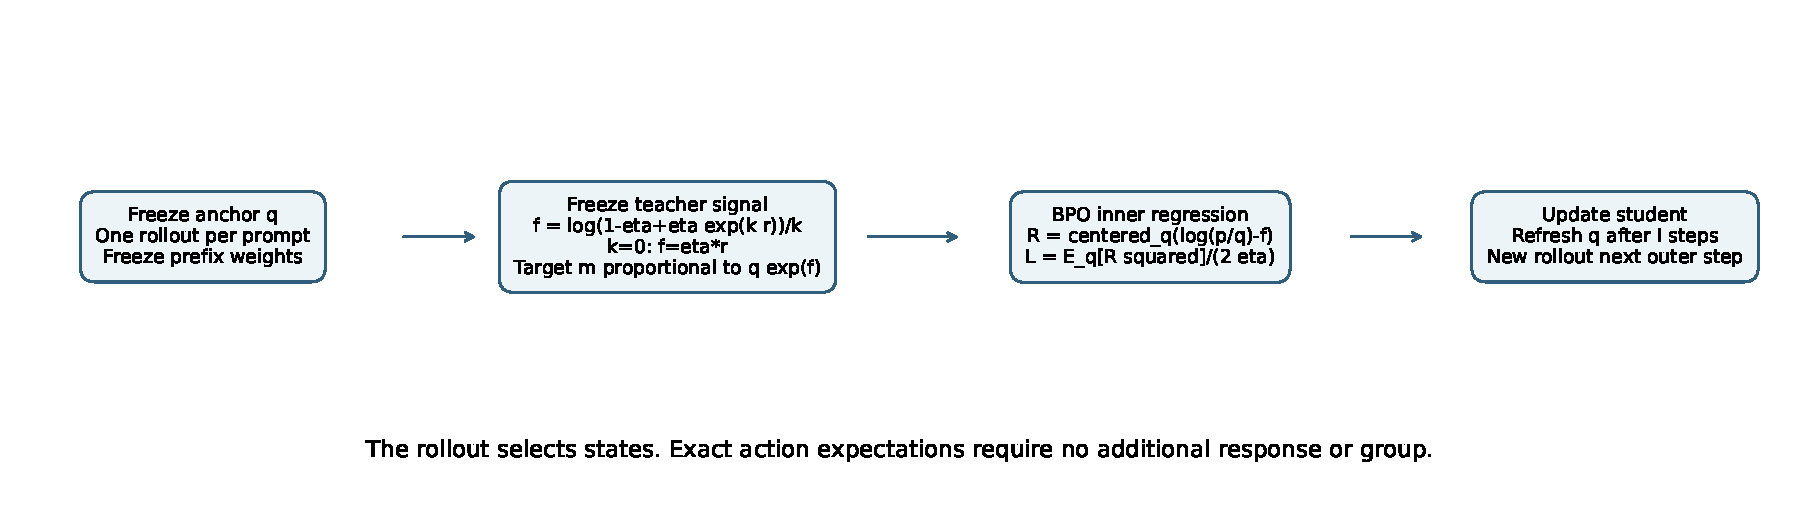
\includegraphics[width=\textwidth]{../../results/power-bpo-algorithm/pipeline.pdf}
 \caption{一条 response 选择前缀，幂均值形状决定冻结监督，BPO 以冻结 $q$ 的条件方差拟合。完整词表求和不需要增加 response 数量。}
\end{figure}
\begin{figure}[htbp]
 \centering
 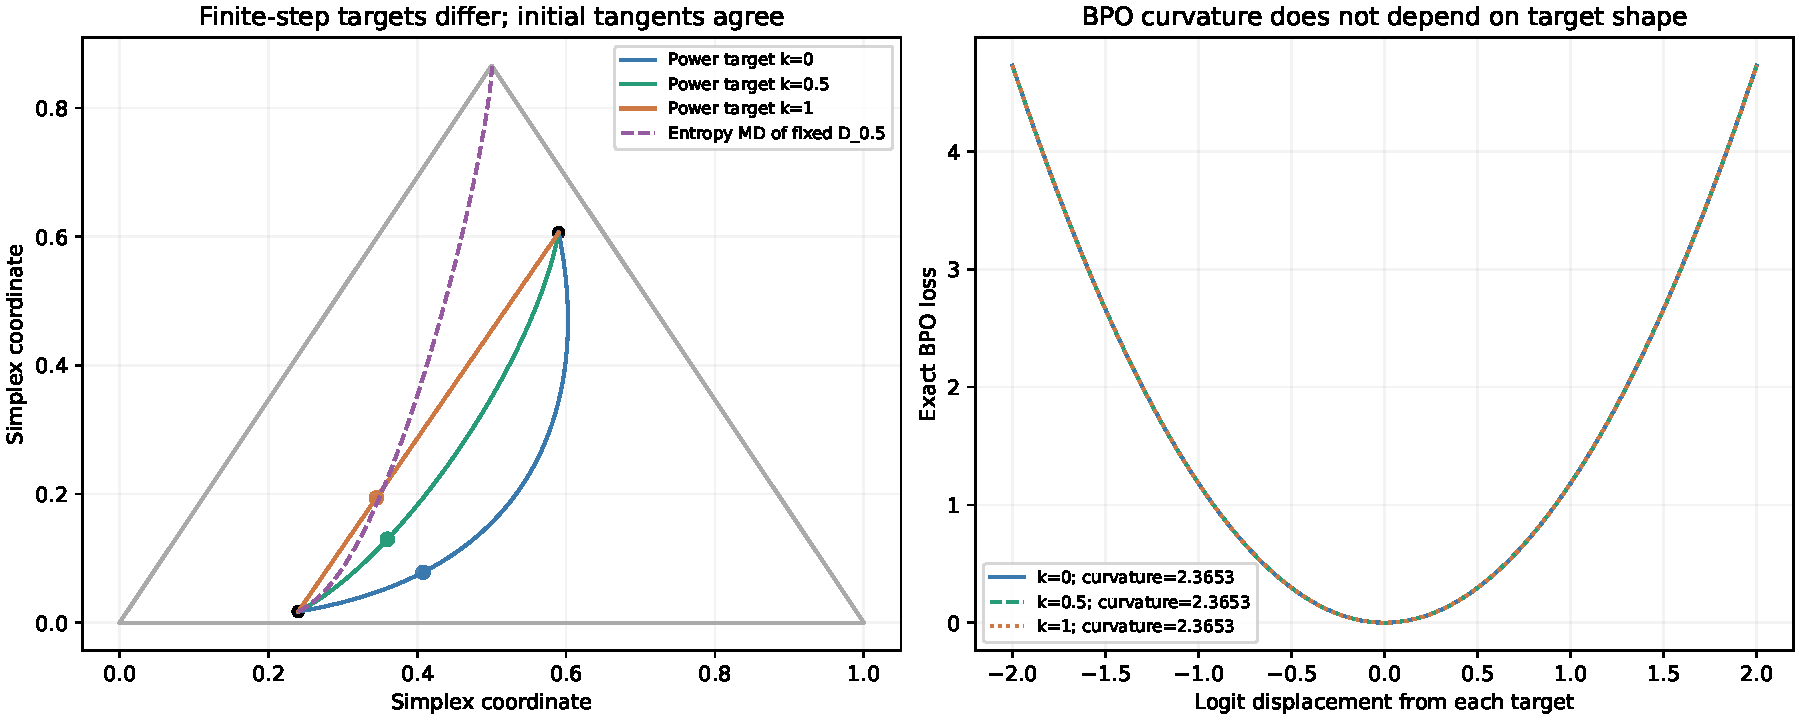
\includegraphics[width=\textwidth]{../../results/power-bpo-algorithm/geometry-and-curvature.pdf}
 \caption{左：幂均值有限步路径与固定 $D_{1/2}$ 的 entropy MD 路径只有起始切向量一致。右：不同 target 只平移固定 $q,\eta$ 的 BPO 二次损失，曲率不随 $\kappa$ 改变。}
\end{figure}
